\documentclass{article}

\usepackage{graphicx}
\usepackage{tikz}
\usepackage{tikzsymbols}
\usetikzlibrary{calc,patterns,shapes.geometric}
\pagestyle{empty}
\usepackage[margin=0pt]{geometry}
\geometry{papersize={14in,12in}}

\def\centerarc[#1](#2)(#3:#4:#5){\draw[#1] ($(#2)+({#5*cos(#3)},{#5*sin(#3)})$) arc (#3:#4:#5);}

\begin{document}
	\begin{figure}
		\centering
		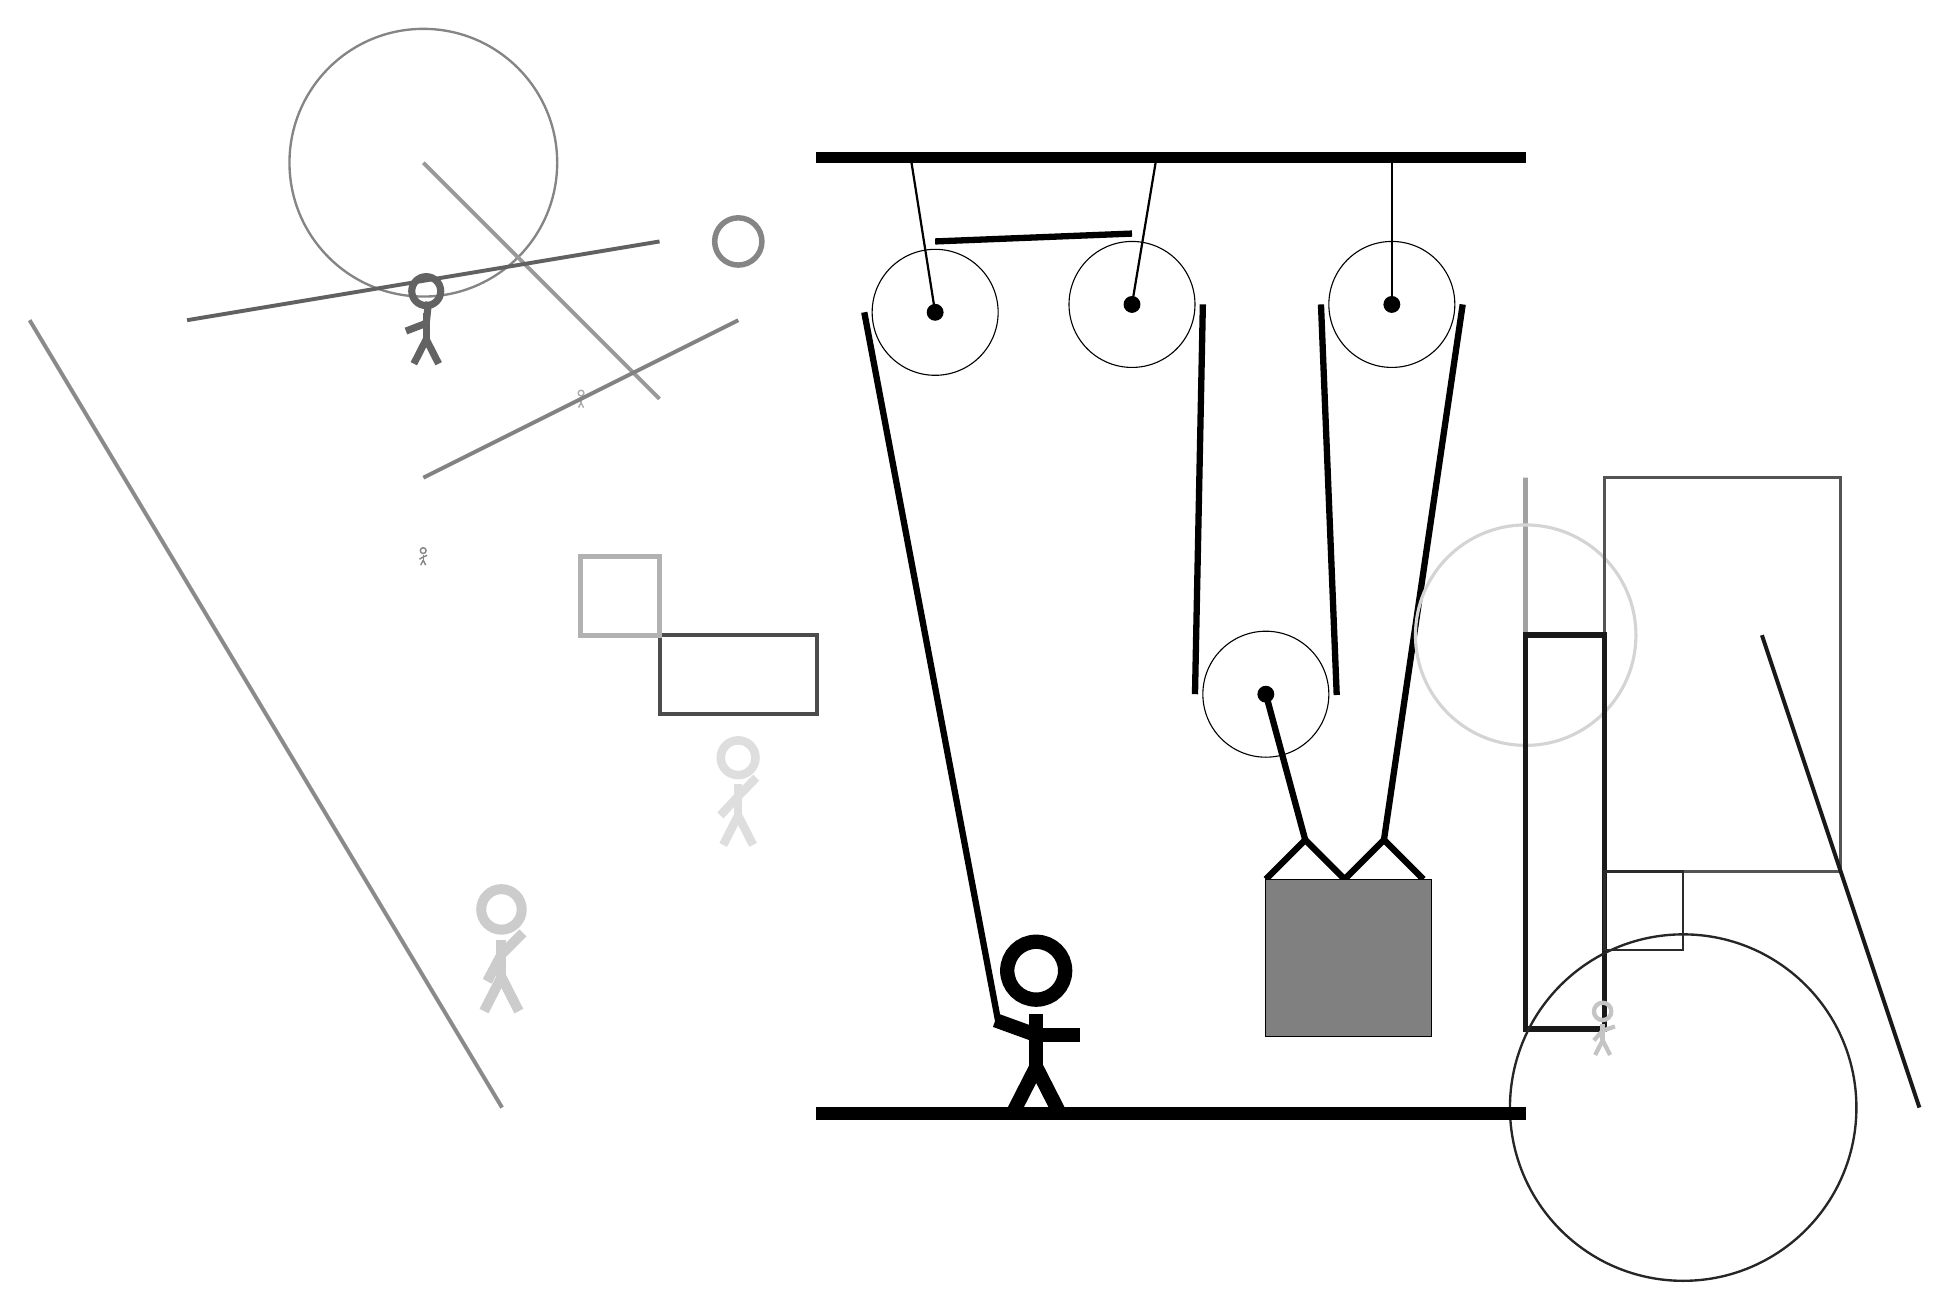
\begin{tikzpicture}
			%%%%% START %%%%%
			
			\draw[fill=black] (-3, 9) rectangle (6, 9.125);
			
			\draw (1, 7.2) circle (0.8);
			\draw[fill=black] (1, 7.2) circle (0.1);
			\draw[thick] (1, 7.2) -- (1.3, 9);
			
			\draw (4.3, 7.2) circle (0.8);
			\draw[fill=black] (4.3, 7.2) circle (0.1);
			\draw[thick] (4.3, 7.2) -- (4.3, 9);
			
			\draw (2.7, 2.25) circle (0.8);
			\draw[fill=black] (2.7, 2.25) circle (0.1);
			
			\draw[line width=0.8mm]  (2.7, -0.1) -- (3.2, 0.4) -- (3.7, -0.1) -- (4.2, 0.4) -- (4.7, -0.1);
			\draw[fill=black!50] (2.7, -0.1) rectangle (4.8, -2.1);
			
			\draw (-1.5, 7.1) circle (0.8);
			\draw[fill=black] (-1.5, 7.1) circle (0.1);
			\draw[thick] (-1.5, 7.1) -- (-1.8, 9);
			
			\draw[line width=0.8mm](-0.7, -1.9) --  (-2.4, 7.1);
			\centerarc[line width=0.8mm](-1.5, 7.1)(90:180:0.9);
			\draw[line width=0.8mm](-1.5, 8.0) -- (1, 8.1);
			\centerarc[line width=0.8mm](1, 7.2)(0:90:0.9);
			\draw[line width=0.8mm](1.9, 7.2) -- (1.8, 2.25);
			\centerarc[line width=0.8mm](2.7, 2.25)(180:370:0.9);
			\draw[line width=0.8mm] (3.6, 2.24) -- (3.4, 7.2);
			\centerarc[line width=0.8mm](4.3, 7.2)(0:180:0.9);
			\draw[line width=0.8mm](4.2, 0.4) -- (5.2, 7.2);
			\draw[line width=0.8mm] (3.2, 0.4) -- (2.7, 2.25);
			
			\node at (-0.2, -2) {\Strichmaxerl[10][-20][0]};
			
			\draw[line width=0.5mm, color=black!46](-7, -3) -- (-13, 7);
			
			\draw[line width=0.5mm, color=black!70] (-5, 2) rectangle (-3, 3);
			\draw[line width=0.7mm, color=black!37] (6, 5) rectangle (6, 2);
			\draw [line width=0.4mm, color=black!17](6, 3) circle (1.4);
			\draw [line width=0.3mm, color=black!48](-8, 9) circle (1.7);
			\draw[line width=0.5mm, color=black!40](-5, 6) -- (-8, 9);
			\draw[line width=0.3mm, color=black!67] (7, 5) rectangle (10, 0);
			\draw[line width=0.5mm, color=black!90](9, 3) -- (11, -3);
			\node[line width=0.5mm, color=black!20] at (-7, -1) {\Strichmaxerl[7][62][45]};
			\draw[line width=0.7mm, color=black!90] (6, -2) rectangle (7, 3);
			
			\draw [line width=0.3mm, color=black!85](8, -3) circle (2.2);
			\node[line width=0.2mm, color=black!61] at (-8, 7) {\Strichmaxerl[5][21][84]};
			\node[line width=0.5mm, color=black!13] at (-4, 1) {\Strichmaxerl[6][47][46]};
			
			\node[line width=0.7mm, color=black!48] at (-8, 4) {\Strichmaxerl[1][30][23]};
			\draw[line width=0.6mm, color=black!30] (-5, 4) rectangle (-6, 3);
			\draw[line width=0.3mm, color=black!83] (8, -1) rectangle (7, 0);
			\node[line width=0.4mm, color=black!32] at (-6, 6) {\Strichmaxerl[1][32][42]};
			\draw [line width=0.7mm, color=black!48](-4, 8) circle (0.3);
			\draw[line width=0.5mm, color=black!62](-5, 8) -- (-11, 7);
			\draw[line width=0.5mm, color=black!49](-8, 5) -- (-4, 7);
			\node[line width=0.5mm, color=black!23] at (7, -2) {\Strichmaxerl[3][48][19]};
			
			
			\draw[fill=black] (-3, -3) rectangle (6, -3.15);
			
			%%%%% END %%%%%
		\end{tikzpicture}
	\end{figure}	
\end{document}